In this new chapter, we continue to drop some of the assumptions we've made so far and generalize the previously introduced model. One of the first assumption we made was that of restricting one item per machine. From now one however, not only one item can be produced by multiple machines but also one machine can produce multiple items. 

\section{Basis of the generalization}

Given that a machine $m$ can now produce more than one item, we introduce the production flow of item $i$ given by machine $m$, which we denote by $X(i,m)$, so that the overall production rate of item $i$ for the plant is given by \[ X(i) = \sum_m X(i,m) \]
What's more, we introduce the coefficient $\lambda(i,m), \forall i, \forall m$ which represents the contribution of machine $m$ in the overall production of item $i$. This contribution, expressed in percentage, is found as \[ \lambda(i,m) = \frac{X(i,m)}{X(i)} \] and it holds that $\sum_m \lambda(i,m) = 1$. 

As well, a direct generalization of what have been done previously gives the utilization of machine $m$ for producing item $i$ as \[ u(i,m) = \frac{X(i,m)}{\mu(i,m)} \] where $\mu(i,m)$ is a given data representing the maximum production rate of machine $m$ for item $i$. 

\begin{figure}[h!]
    \centering
    \begin{tikzpicture}
        \draw[->] (0,0) -- (10, 0);
        \draw (0,0) rectangle node {$"1"$} (2, .5);
        \draw (1, 1) node {$T_1$};

        \draw (3,0) rectangle node {$"3"$} (5, .5);
        \draw (4, 1) node {$T_2$};

        \draw (5, 0) rectangle node {$"1"$} (6, .5);
        \draw (5.5, 1) node {$T_3$};

        \draw (6.5, 0) rectangle node {$"2"$} (8, .5);
        \draw (7.25, 1) node {$T_4$};

        \draw (8, 0) rectangle node {$"3$} (9.5, .5);
        \draw (8.75, 1) node {$T_5$};

        \draw[decorate, decoration={brace, amplitude=5pt}] (10, -.2) -- (0, -.2);
        \draw (4.5, -.7) node[right] {$\sum T = \sum T_i + \textrm{idle time}$};

        \draw (13, 1) node {$u(1,m) = \dfrac{T_1 + T_3}{\sum T}$};
        \draw (13, 0) node {$u(2,m) = \dfrac{T_4}{\sum T}$};
        \draw (13, -1) node {$u(3,m) = \dfrac{T_2 + T_5}{\sum T}$};

    \end{tikzpicture}
    \caption{\label{shared_res:util}Machine utilisation with respect to a given item}
\end{figure}

From the example represented in figure (\ref{shared_res:util}), we can easily understand that $\sum_i u(i,m) \le 1$ (which basically means that a machine cannot be utilized more than its maximum production capacity). By substituting the newly introduced quantities in that inequality, and keeping in mind that $X(i) = X_fn_{if}$, it holds that
\[
    \begin{split}
        \sum_i u(i,m) \le 1, \forall m &\Leftrightarrow \sum_i\frac{X(i,m)}{\mu(i,m)} \le 1, \forall m\\
        \Leftrightarrow& \sum_i\frac{X(i)\lambda(i,m)}{\mu(i,m)} \le 1, \forall m\\
        \Leftrightarrow& \sum_i\frac{X_fn_{if}\lambda(i,m)}{\mu(i,m)} \le 1, \forall m\\
    \end{split}
\]
And since this set of inequality has to be fullfilled for every machine, then it holds that the only way to satisfy them all is to select $X_f$ as \begin{equation} X_f\le\min_m\left( \dfrac{1}{\sum_i\frac{n_{if}\lambda(i,m)}{\mu(i,m)}} \right) \label{shared_res:eqn_xfmax} \end{equation}

Note how, in the case of a single machine per item (i.e. $i=m$), it holds that $\lambda(i,m) = 1, \forall i=m$ and $0$ otherwise so that the minimum among all the machines becomes equivalent to the minimum among the items in such a way that the freshly established formula can be written as 
\[
    \min_m\left( \dfrac{1}{\sum_i\frac{n_{if}\lambda(i,m)}{\mu(i,m)}} \right) \overset{i=m}{=} \min_i\left( \dfrac{1}{ \frac{n_{if}}{\mu_i} } \right) = \min_i\left( \frac{\mu_i}{n_{if}} \right)
\] which is the formula we had found so far. 

\section{Model without setup time consideration}

If we do not consider the setup time of each machine, it still holds that $\mu(i,m) = \frac{1}{T_o(i,m)}$ which leads to the simplified following expression :
\begin{equation} X_f^{max}(\lambda) = \min_m\left( \frac{1}{ \sum_in_{if}\lambda(i,m)T_o(i,m) } \right) \label{shared_res:eqn_xf_wthout_setup} \end{equation} Thus, to determine the overall maximum production rate, one has to maximize, among all admissable values of $\underline\lambda$, the above expression. The problem can then be stated as follow : 
\[
    \begin{split}
        \underset{\underline\lambda}{\textrm{maximize }}& \min_m\left( \frac{1}{\sum_in_{if}\lambda(i,m)T_o(i,m)} \right)\\
        \textrm{subject to }& \sum_m \lambda(i,m) = 1, \forall i
    \end{split}
\]

\begin{wrapfigure}[10]{r}{4cm}
    \centering
    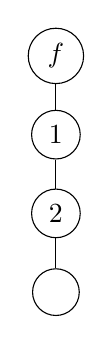
\begin{tikzpicture}[scale=.5]
        \draw (0,0) node[circle, draw] (f) {$f$};
        \draw (0,-2) node[circle, draw] (1) {$1$};
        \draw (0,-4) node[circle, draw] (2) {$2$};
        \draw (0,-6) node[circle, draw] (RM) {$\vphantom{f_i}$};

        \draw (RM) -- (2);
        \draw (2) -- (1);
        \draw (1) -- (f);
    \end{tikzpicture}
    \caption{\label{shared_res:bom1} Example}
\end{wrapfigure}

Let's consider the bill of material represented in figure (\ref{shared_res:bom1}) which depicts an assembly line. Two machines are present in the plant. The first machine, denoted $M_1$, can produce product $f$ and $1$ while the second one, $M_2$, can produce the products $1$ and $2$. The operational times of each machine for a given product are the following :
\begin{align*}
    T(f, M_1) &= 10 & T(1, M_1) &= 3 & T(2, M_2) &= 10 & T(1, M_2) &= 5
\end{align*}

Since some products can only be produced by specific machines, we can deduce some of the values of $\underline\lambda$. Indeed, it is clear that $\lambda(f,M_1) = 1$ and $\lambda(2, M_2) = 1$ and that $\lambda(f, M_2) = 0$ and $\lambda(2, M_1) = 0$. As regarding to the undetermined coefficients, we can at least, say that $\lambda(1, M_1) = 1 - \lambda(1, M_2)$ holds since product $1$ can be produced by both $M_1$ and $M_2$. Let's denote by $\lambda$ an arbitrary chosen coefficient among these two, let's say, $\lambda = \lambda(1, M_1)$. We can now compute the maximum production rate using equation (\ref{shared_res:eqn_xf_wthout_setup}) as follow :
\[
    X_f^{max}(\lambda) = \min\left( \frac{1}{1.10 + \lambda.3 + 0} ; \frac{1}{0+(1-\lambda).5+1.10} \right) = \min\left( \frac{1}{10+3\lambda} ; \frac{1}{15-5\lambda} \right)
\]
which is the function of $\lambda$ to be maximized. As it can  be seen in figure (\ref{shared_res:max_min_wthout_setup}), we have to maximize the function represented by a thick line which corresponds to the above computation. It is clear that the maximum is reached at the intercept of the two lines which is computed as \[ 3\lambda + 10 = 15 - 5\lambda\Leftrightarrow \lambda^\circ = \frac{5}{8} \] for which we find that \[ X_f^{max} = X_f^{max}(\lambda^\circ) = \frac{1}{3.\frac{5}{8}+10} = \frac{8}{95} \]

\begin{figure}[h!]
    \centering
    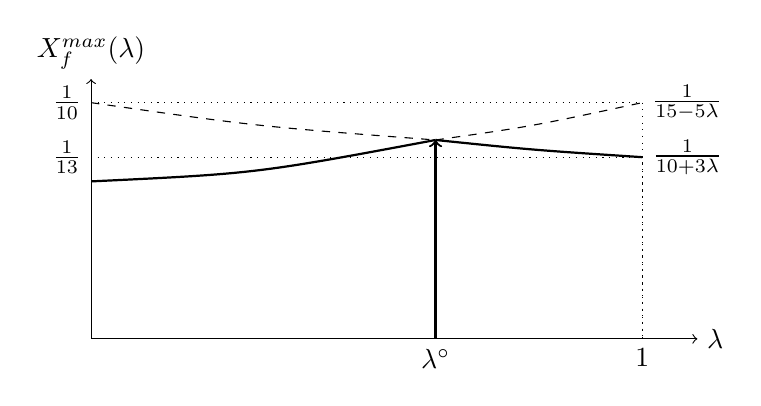
\begin{tikzpicture}[yscale=30, xscale=7]
        \draw[<->] (0, .11) node[above] {$X_f^{max}(\lambda)$} |- (1.1, 0) node[right] {$\lambda$};
        
        \draw[dotted] (0, .1) node[left] {$\frac{1}{10}$} -| (1, 0);
        \draw[dotted] (0, 1 / 13) node[left] {$\frac{1}{13}$} -| (1, 0) node[below] {$1$};

        \draw[thick] (0, 1/15) .. controls (.3, .07) .. (5/8, 8/95);
        \draw[dashed] (5/8, 8/95) .. controls (.8, .09) .. (1, .1) node[right] {$\frac{1}{15-5\lambda}$};

        \draw[thick] (5/8, 8/95) .. controls (.8, .08) .. (1, 1/13) node[right] {$\frac{1}{10+3\lambda}$};
        \draw[dashed] (0, .1) .. controls (.3, .09) .. (5/8, 8/95);

        \draw[->, thick] (5/8, 0) node[below] {$\lambda^\circ$} -- (5/8, 8/95);

    \end{tikzpicture}
    \caption{\label{shared_res:max_min_wthout_setup}Maximizing the minimum to find $X_f^{max}$}
\end{figure}

\section{Model with setup time (sequence independent)}

In this section, we add consideration for setup times with a simplifying assumption which is that setup times do not depend on the sequence of the items produced on one machine. This may not always be the case however. 

Similarly to what have been done when we firstly introduced the setup time in the second chapter, we can still consider the following to hold, with direct generalization : 
\begin{center}
    \begin{tikzpicture}
        \draw[->] (0, 0) node[left] {$m$} -- (5, 0);
        \draw[dotted] (.5, 0) rectangle (2, .5);
        \path (.5, .5) rectangle node {$T_{sm}$} (2, 1);
        \draw (2, 0) rectangle node {$b(i,m)$} (4.5, .5);

        \draw (8, .5) node {$\mu(i,m) = \dfrac{ b(i,m) }{ T_{sm} + b(i,m)T_o(i,m) }$};
    \end{tikzpicture}
\end{center}
Which yields from equation (\ref{shared_res:eqn_xfmax})
\[
    \begin{split}
        X_f^{max}(\underline\lambda, \underline b)
        &= \min_m\left( \frac{1}{ \sum_i\frac{ n_{if}\lambda(i,m)(T_{sm}+b(i,m)T_o(i,m)) }{b(i,m)} } \right)\\
        &= \min_m\left( \frac{1}{T_{sm}\sum_i\frac{n_{if}\lambda(i,m)}{b(i,m)} + \sum_i n_{if}\lambda(i,m)T_o(i,m)} \right)
    \end{split}
\] where $X_f^{max}$ is a function of $\underline\lambda$ and $\underline b$. We then have three possible cases :
\begin{itemize}
    \item Having fixed $\underline\lambda$, we can maximize $X_f^{max}$ with respect to $\underline b$. This bound is denoted by $\bar X_f^{max}(\underline\lambda) = \max_{\underline b}X_f^{max}(\underline\lambda, \underline b)$. Looking at the expression of $X_f^{max}$, one can notice that $\underline b$ appears only in one of the two term of the main sum, at the denominator. Thus, maximizing $X_f^{max}$ with respect to $\underline b$, having fixed $\underline\lambda$, can be done by assigning to $\underline b$ its maximum value $\underline b^{max}$.
    \item Having fixed $\underline b$, we can maximize $X_f^{max}$ with respect to $\underline \lambda$. This bound is denoted $\bar\bar X_f^{max}(\underline b) = \max_{\underline\lambda}X_f^{max}(\underline\lambda, \underline b)$
    \item Looking for the overall maximum production rate, we have to maximize $X_f^{max}$ with respect to both $\underline\lambda$ and $\underline b$. This bound is denoted $\bar\bar\bar X_f^{max} = \max_{\underline\lambda, \underline b}X_f^{max}$ which in fact, for the same reasons we have discussed for $\bar X_f^{max}$, can be computed as $\max_{\underline\lambda}\bar X_f^{max}(\underline\lambda)$
\end{itemize}

\section{A worked example}

